%Grundsätzliches: Enthalten sind die Gebieten die Frau Baumann schon als Schwerpunkte angekündigt hat (und natürliche das nicht ausdrücklich geforderte Grundwissen auf dem sie aufbauen).
%Das meiste ist eher knapp gehalten, extrem grundlegende Dinge wie "was ist eine Linearkombination", "wie addiert man Matrizen" etc. sind nicht nochmal erklärt weil ich denke dass das beim lernen eher stört.
%Selbstverständlich kannst du auch noch kürzen/ergänzen 

\documentclass[10pt,a4paper]{article}
\usepackage[utf8]{inputenc}
\usepackage{amsmath}
\usepackage{amsfonts}
\usepackage{amssymb}
\usepackage{graphicx}
\usepackage[margin=0.6in]{geometry}
\begin{document}
\section*{\textit{Prüfungsrelevante} Verfahren, Sätze und Rechenregeln}
\section{Lineare Algebra}



\subsection{Komplexe Zahlen}
\begin{itemize}
\item $z=a+bi \in \mathbb{C}$ (\textbf{arithmetische} Darstellung)
\item $(\mathbb{C},+,\cdot)$ ist Körper der komplexen Zahlen (+ hat neutrales Element 0 und inverses Element $-z$; $\cdot$ hat neutrales Element 1 und inverses Element $z^{-1}$; beide assoziativ und kommutativ; $\cdot$ distributiv über +)
\item $\dfrac{z_{2}}{z}=\dfrac{z_{2}}{z}\cdot \dfrac{\overline{z}}{\overline{z}}=\dfrac{z_{2}\cdot \overline{z}}{a^2+b^2},\; \text{Re}(z)=a, \; \text{Im}(z)=b, \; \overline{z}=a-bi,\; r[\text{cos}(\varphi)+i\cdot \text{sin}(\varphi)]=re^{i\varphi}$
\item $r=\sqrt{a^2+b^2},\; \text{sin}(\varphi)=\dfrac{a}{r}, \;\text{cos}(\varphi)=\dfrac{b}{r}$; ob arccos oder arcsin zur Bestimmung von $\varphi$ zu verwenden ist wird aus Vorzeichen von $\frac{a}{r}$ bzw. $\frac{b}{r}$ klar 

%noch genauer ausführen!

\item \textbf{trigonometrische} und \textbf{eulersche} Darstellung erfolgt geometrisch in Polarkoordinaten $z=(r,\varphi)$
\end{itemize}
\begin{center}
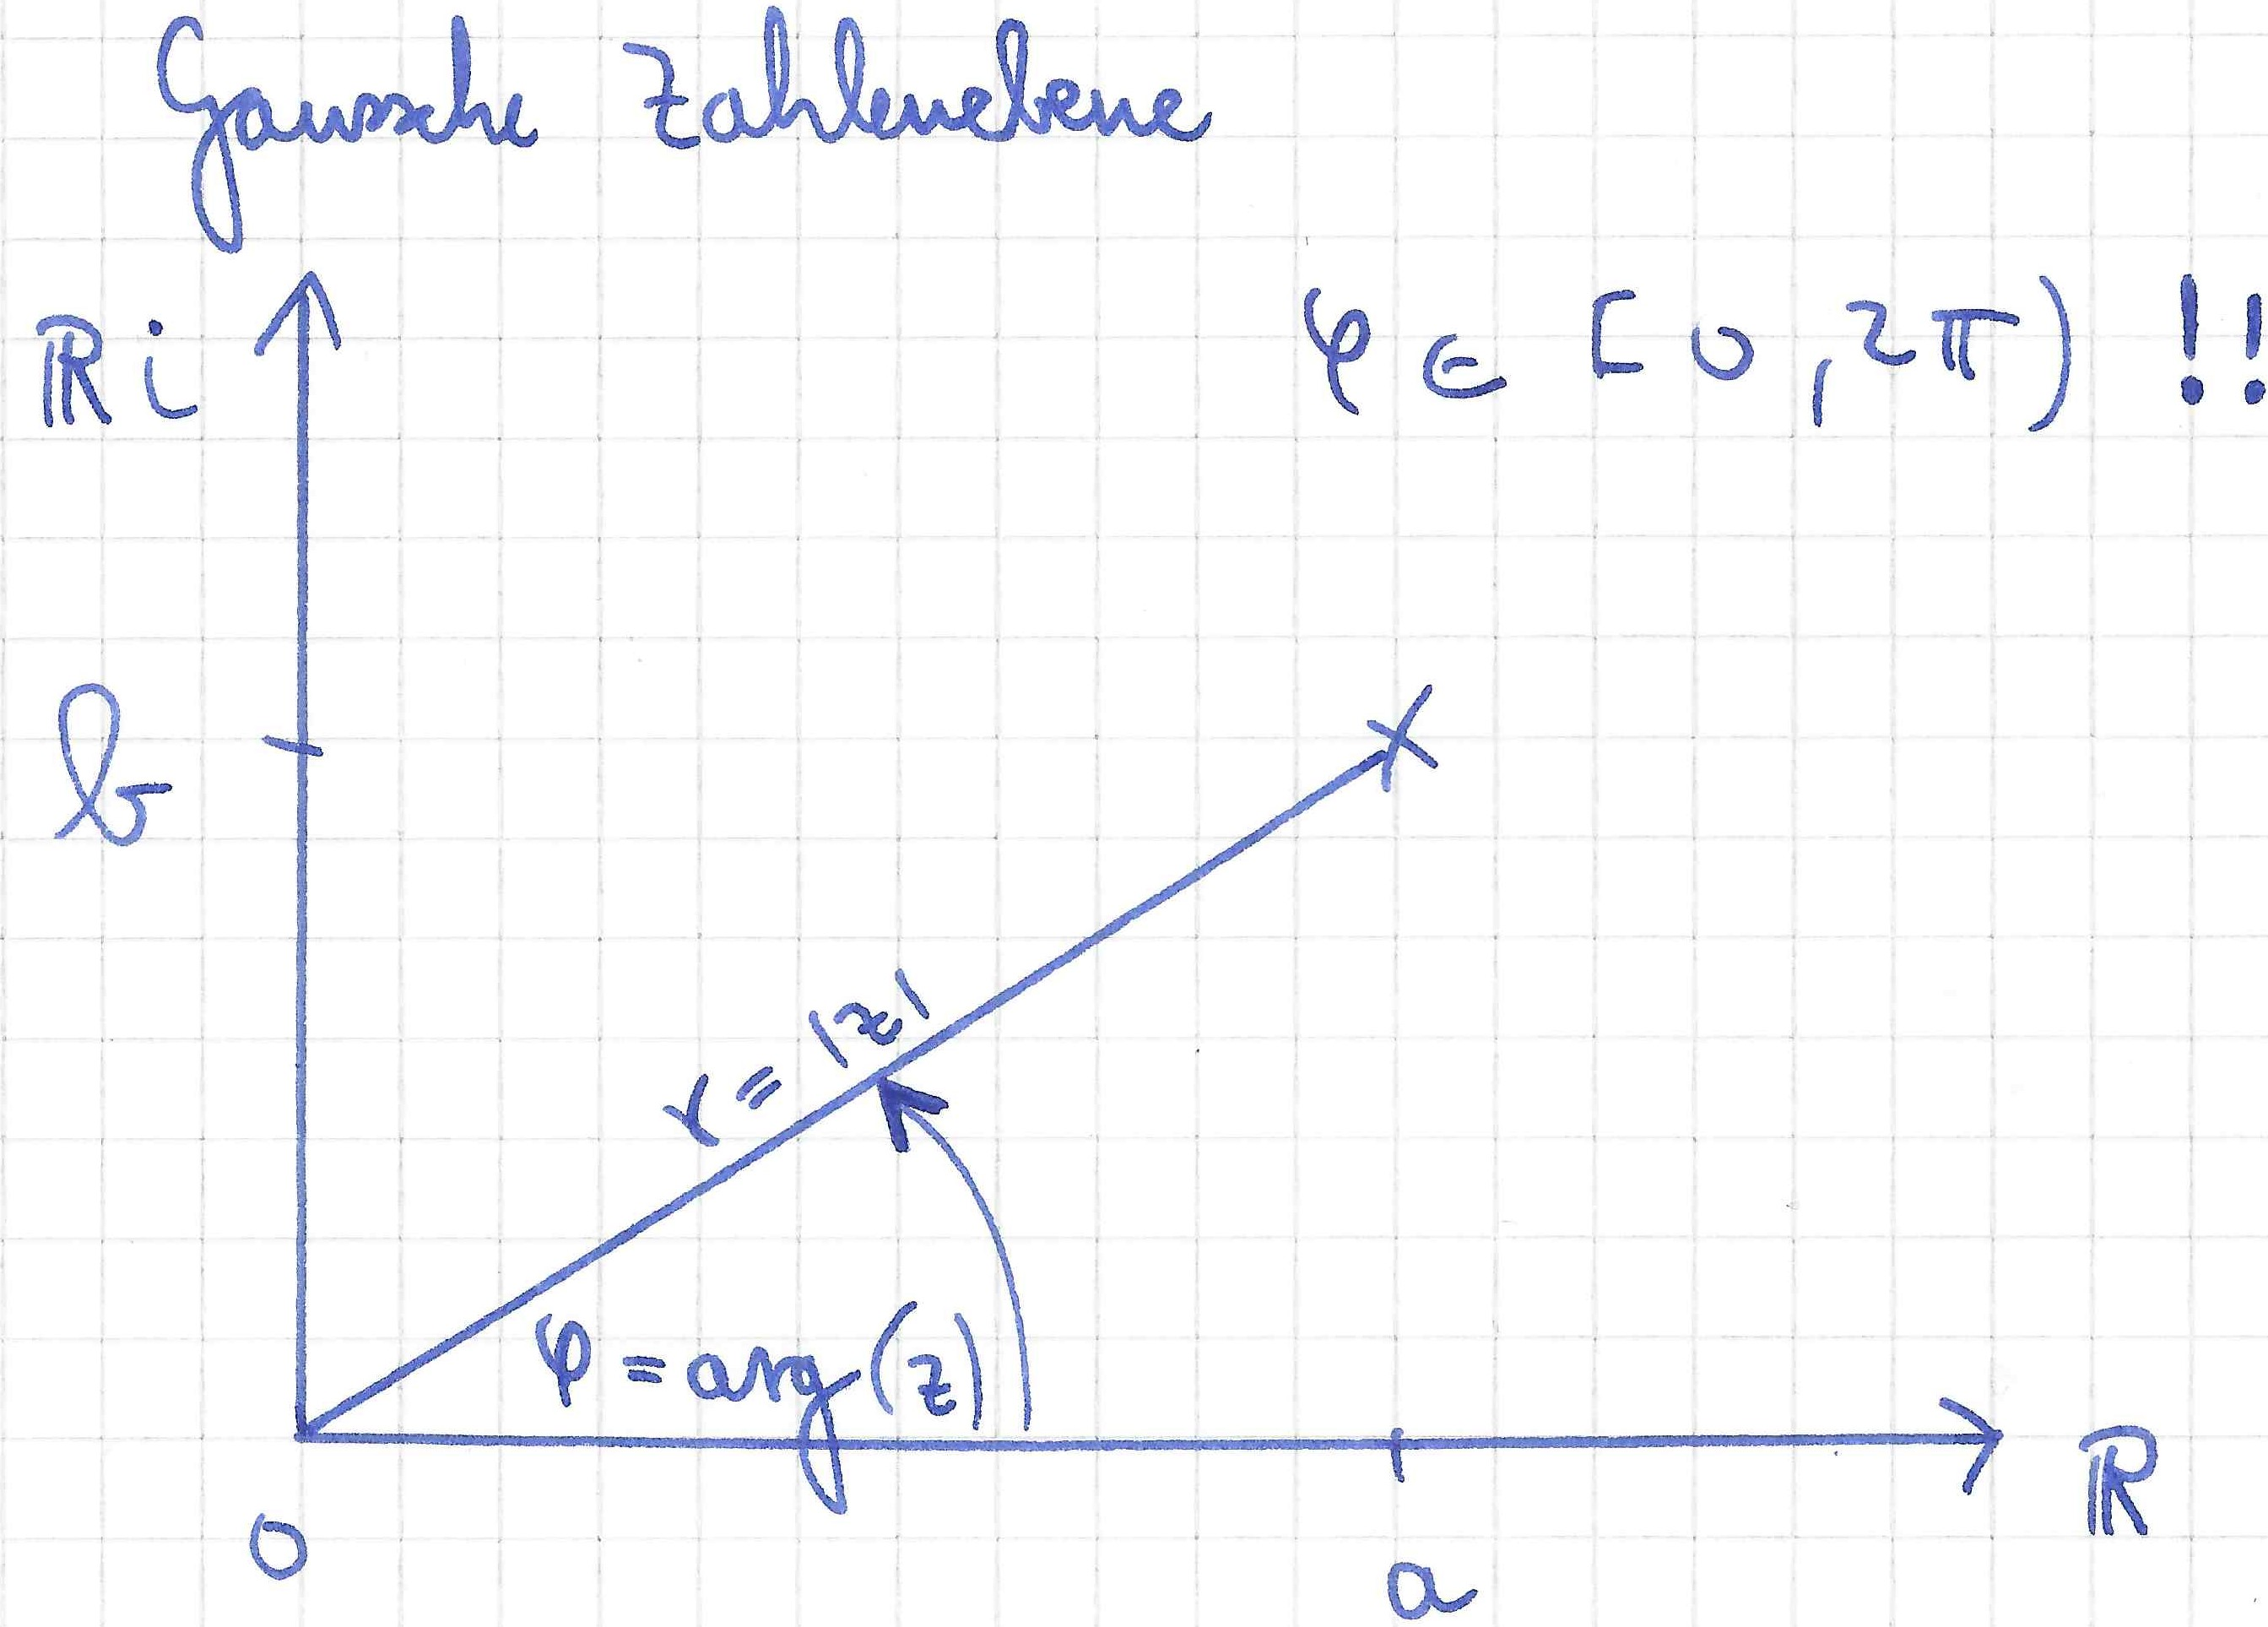
\includegraphics[scale=0.55]{Gaussche Zahlenebene.jpg}\\
\textit{für komplexe Zahlen sind auch einfache Beweise prüfungsrelevant, rechnen mit euler/trig jedoch nicht}
\end{center}



\subsection{Rechnen mit Matrizen}
\begin{itemize}
\item Matrizen sind Abbildungen die einem Paar $(i,j)$ ein Körperelement $a_{ij}$ zuordnen 
\item Matrix $A=(a_{ij})=(a_{ij})_{m \times n}$, es gibt $i$ horizontale Zeilen und $j$ vertikale Spalten; Hauptdiagonale von links oben nach rechts unten
\item spezielle Matrizen: Einheitsmatrix, Nullmatrix, quadratische Matrix (auch "n-reihig") und Diagonalmatrix (quadratisch und $a_{ij}=0$ für $i\neq j$)
\item Matrixmultiplikation: $(a_{ij})_{m\times n} \cdot (b_{ij})_{n \times p}=(\sum_{k=1}^{n} a_{ik}\cdot b_{kj})_{m \times p}$ 
\item $A^{T}$: Zeilen und Spalten vertauschen
\item + kommutativ mit neutralem Element Nullmatrix; $\cdot$ assoziativ mit neutralem Element Einheitsmatrix und Nullmatrix absorbiert; $\cdot$ distributiv über + 
\item $(A+B)^{T}=A^{T}+B^{T},\; (kA)^{T}=kA^{T},\; (A^{T})^{T}=A,\; (A\cdot B)^{T})=B^{T}\cdot A^{T}$ (Reihenfolge !!)
\item $A^{-1}$ ist zu ermitteln durch $(A\mid E_{n})\rightsquigarrow (A \text{ in ZSF} \mid E_{n}') \rightsquigarrow (E_{n} \mid A^{-1})$ mit elementaren Zeilenumformungen\\ $A$ in ZSF hat keine Nullzeile $\Leftrightarrow\text{rg}(A)= n \Leftrightarrow\text{dim Ker}(A)=0\Leftrightarrow \text{det}(A)\neq 0 \Leftrightarrow \exists A^{-1}$ 
\item $A\in \mathbb{R}^{2\times 2} \Rightarrow A^{-1}=\text{det}(A)^{-1}\cdot \begin{pmatrix} d& -b\\ -c&a\end{pmatrix}$
\end{itemize}



\subsection{LGS und Gauß-Jordan}
\begin{itemize}
\item GF2=$\left\lbrace 0,1\right\rbrace$, + und $\cdot$ für GF2 wie in $\mathbb{R}$ mod 2 ($\Rightarrow -a=a$)
\item \textbf{homogenes} LGS: alle unveränderlichen sind 0, Nulltupel ist immer eine Lösung; \textbf{inhomogenes} LGS: mindestens eine unveränderliche ist verscheiden von 0, Nulltupel keine Lösung  
\item Matrixschreibweise für LGS: $A\overrightarrow{x}=\overrightarrow{b}$, Kurzform: Koeffizientenmatrix $(A \mid b)$
\item für LGS in \textbf{ZSF} (ZSF ist am besten am Beispiel zu verstehen, siehe Folie 3.7) gilt: $L=\emptyset \Leftrightarrow \exists b$ in einer Nullzeile das verschieden von 0 ist; umgekehrt für $L\neq \emptyset$
\item aus \textbf{reduzierter ZSF} (siehe Folie 3.9) kann man Lösung direkt ablesen; um (reduzierte) ZSF zu erhalten nutzt man \textbf{elementare Zeilenumformungen}: Zeilen vertauschen, Zeile mit $k\in K\setminus \left\lbrace 0\right\rbrace$ multiplizieren, k-faches einer Zeile zu anderer addieren
\item Gauss: LGS in ZSF, Lösbarkeitsentscheidung; Jordan: LGS in reduzierte ZSF
\item Nullzeilen dürfen weggelassen werden, Spalten dürfen vertauscht werden (Variablennamen dranschreiben!)
\item notieren der Lösungsmenge z.B. als $L=\left\lbrace (2,3t,1,5k)\mid t,k \in K \right\rbrace$ oder als Menge von (hier 3) Vektoren, evtl. auch als Spanraum; so oder so Probe nicht vergessen!
\item GF2 LGS mit n Parametern in der Lösungsmenge hat $2^{n}$ konkrete Lösungen ($\mathbb{C}/\mathbb{R}$ LGS unendlich viele)
\end{itemize}



\subsection{Vektorräume (VR)}
\begin{itemize}

%VR Axiome sollten nicht auswendig nötig sein

\item K-VR= algebraische Struktur $(V; \oplus , \underbrace{(k \mid k \in K)}_{\text{Skalarmultiplikation}})$ \textit{(beachte wo ; und wo , steht),} muss VR-Axiome erfüllen
\item zu Unterscheiden sind $0_{v}$ und $0_{k}$, beide eindeutig bestimmt 
\item $kv=0_{v} \Leftrightarrow k=0_{k} \lor v=0_{v},\;\;\; (-k)v=\ominus kv, \;\;\; (-1)v=\ominus v\;\;\;\;$ (nach V5 ist $\ominus v$ Inverses von v)
\item $U$ heißt \textbf{Untervektorraum} (UVR) von V wenn: 
\begin{enumerate} 
\item $0_{v} \in U$
\item $a,b\in U \Rightarrow a\oplus b \in U$ für alle $a,b \in U$ (abgeschlossen bzgl. $\oplus$)
\item $a\in U, k\in K \Rightarrow ka \in U$ für alle $a\in U,k\in K$ (abgeschlossen bzgl. $\odot$)
\item ($U\subseteq V$, immer zuerst prüfen!)
\end{enumerate}
\item $U_{1},U_{2}$ UVR von $V \Rightarrow U_{1} \cap U_{2}$ UVR von $V$
\end{itemize} 
\textit{VR Axiome nachweisen nicht prüfungsrelevant}



\subsection{Spanräume und Basen}
\begin{itemize}
\item für $T\subseteq V$ ist Span$(T)=\langle T \rangle$ der kleinste UVR der $T$ enthält \item Berechnung: Span$(\left\lbrace v_{1},\dotsc ,v_{n}\right\rbrace)=\left\lbrace k_{1}v_{1}\oplus \dotsc \oplus k_{n}v_{n}\mid k_{1},\dotsc ,k_{n} \in K\right\rbrace $
\item $\langle V\rangle =V, \;\; \langle \emptyset \rangle =\left\lbrace 0_{v} \right\rbrace,\;\;$ für $T\subseteq V,V=$ Span$(T)$ ist T \textbf{Erzeugendensystem} von V
\item Möglichkeiten zum Prüfen ob $T=\left\lbrace  v_{1}, \dotsc, v_{n} \right\rbrace$ z.B. Erzeugendensystem des $\mathbb{R}^{3}$ ist: 
\begin{enumerate}
\item gibt es überhaupt dim$(\mathbb{R}^3)=3$ lin. u. Vektoren in $T$?
\item ist LGS $\left(v_{1} \dotsc v_{n} \mid \begin{matrix} a\\  b\\c\end{matrix}\right)$ lösbar? 
\end{enumerate}
\item für eine \textbf{Basis} $B$ von $V$ gilt: $B$ ist lin. u. und $V=\text{Span}(B)$; alternativ kann geprüft werden: \begin{enumerate}
\item $B$ ist Erzeugendensystem von $V$, jede echte Teilmenge von $B$ ist kein Erzeugendensystem von $V$
\item $B$ ist lin. u., $B\cup \left\lbrace v \right\rbrace (v \in V,v\not\in B)$ ist lin. a. 
\item für $V$ mit dim$(V)=n$ genügt es zu Prüfen, ob ($B$ Erzeugendensystem mit $\vert B\vert=n$) oder ($B$ lin. u. und $\vert B\vert=n$)
\end{enumerate}
\item zwei Basen von $V$ haben immer die gleiche Mächtigkeit $n=:\, $dim($V$); Basis vom Nullraum ist $\emptyset$
\item ist $B=(b_{1},\dotsc,b_{n})$ \underline{angeordnete} Basis von $V$, so lässt sich $v\in V$ als $v=k_{1}b_{1}\oplus\dotsc  \oplus k_{n}b_{n}$ darstellen und $v_{B}=\begin{pmatrix} k_{1}\\ \vdots\\ k_{n} \end{pmatrix}$ heißt \textbf{Koordinatenvektor} von $v$ bzgl. $B$ 
\end{itemize}



\subsection{Lineare Unabhängigkeit (lin. u. - keine offizielle Abkürzung)}
\begin{itemize}
\item $\left\lbrace v_{1}, \dotsc, v_{n} \right\rbrace$ ist lin. u. wenn gilt: $k_{1}v_{1} \oplus \dotsc \oplus k_{n}v_{n}=0_{v} \Rightarrow k_{1}=\dotsc=k_{n}=0_{k}$ 
\item in einer Menge lin. a. Vektoren kann \textit{mindestens ein} Vektor als LK der anderen dargestellt werden, es können aber i.A. \textit{nicht alle} Vektoren der Menge als LK der jeweils anderen dargestellt werden!
\item einige Möglichkeiten um $M=\left\lbrace v_{1}, \dotsc, v_{n}\right\rbrace$ auf lin. u. zu prüfen:
\begin{enumerate}
\item einfach LGS aufstellen (anders formuliert gilt also Ker$[(v_{1} \dotsc v_{n})]=\left\lbrace 0_{v} \right\rbrace \Rightarrow$ lin .u.)
\item es liegen in allen Vektoren in immer verschiedenen Komponenten Nullen vor $\Rightarrow$ lin. u.\\ (z.B. $\left\lbrace(0,1,0,4)^{T},(0,0,3,0)^{T},(2,0,0,0)\right\rbrace$ lin. u.) 
\item $0_{v} \in M \Rightarrow$ \textit{lin. a.}
\item  dim$(V)=n \Rightarrow$ mehr als $n$ Vektoren sind immer \textit{lin. a.}
\item rg$[(v_{1} \dotsc v_{n})]=n$ bzw. dim(Ker$[(v_{1} \dotsc v_{n})])=0$ bzw. det$[(v_{1} \dotsc v_{n})]\neq 0 \Rightarrow$ lin. u. 
\item $v_{1},\dotsc, v_{n}$ sind paarweise orthogonal $\Rightarrow$ lin. u.
\end{enumerate}

\end{itemize}
\textit{einfache Beweise sind prüfungsrelevant}



\subsection{Eigenschaften von Matrizen und LGS}
\begin{itemize}

%Begriff der affinen Teilräume hier erstmal ignoriert, sollte auch keine Rolle spielen

\item \textbf{Kern} einer Matrix Ker$(A)$ ist Lösungsmenge von $(A\mid \overrightarrow{0})$ (dem zugehörigen homogenen LGS), Ker$(A)$ ist ein VR
\item Lösungsmengen inhomogener LGS sind keine VR; je zwei Lösungen des inhomogenen LGS unterscheiden sich um eine Lösung des homogenen LGS (=Kern der Koeffizientematrix)
\item für $A=(s_{1}\dotsc s_{n})$ ist der \textbf{Spaltenraum} Col$(A)=\text{Span}(\left\lbrace s_{1},\dotsc, s_{n}\right\rbrace)$, dim(Col$(A))$ heißt Spaltenrang (entspricht maximaler Menge lin. u. Spaltenvektoren von A); ganz analog für \textbf{Zeilenraum} Row$(A)$
\item Es gilt dim(Col$(A))$=dim(Row$(A))=:\text{rg}(A)\;\;\;$ (Rang von A); Berechnung: rg$(A)= \#$ nicht-Nullzeilen in ZSF
\item \textbf{Dimensionsformel: }$A\in K^{m \times n}\Rightarrow\text{rg}(A)+\text{dim(Ker}(A))=n$;  Lösbarkeitskriterium: $Ax=b$ lösbar $\Leftrightarrow \text{rg}(A)=\text{rg}(A \mid b)$
\end{itemize}
\textit{$\approx$ Ende LA 110.1}



\subsection{Lineare Abbildungen}
\begin{itemize}
\item sind $(V; \oplus_{V}, (k\mid k\in K)),(W; \oplus_{W}, (k\mid k\in K))$ VR über dem selben Körper, so ist $f:V \rightarrow W$ eine lineare Abbildung wenn:
\begin{enumerate}
\item $f(a \oplus_{V} b) =f(a)\oplus_{V} f(b)$
\item $f(ka)=kf(a)$
\end{enumerate}
%\item $f(k_{1}v_{1}\oplus_{V}\dotsc \oplus_{V} k_{n}v_{n})=\underbrace{k_{1}f(v_{1})\oplus_{W}\dotsc\oplus_{W} k_{n}f(v_{n})}_{\text{LK von Vektoren aus W}}$ 

% line 146 erstmal rauskommentiert weil ist eigentlich klar, und steht so ähnlich auch schon in 157

\item Sei $\left\lbrace b_{1},\dotsc,b_{n}\right\rbrace$ Basis von $V.\;\;\;\;$   \textbf{f injektiv} $\Leftrightarrow \left\lbrace f(b_{1}), \dotsc,f(b_{n}) \right\rbrace $ lin. u. $\Leftrightarrow$ Ker$(f)=\left\lbrace 0_{v} \right\rbrace$
\item \textbf{f surjektiv} $\Leftrightarrow$ Span$(\left\lbrace f(b_{1}), \dotsc,f(b_{n}) \right\rbrace)=W$
\item \textbf{f bijektiv} $\Leftrightarrow \left\lbrace f(b_{1}), \dotsc,f(b_{n}\right\rbrace$ ist Basis von W\\ Für Beweise bzgl. dieser 3 Eigenschaften bieten sich oft Gegenbeispiele an!
\item Ker$(f)=\left\lbrace v \mid v \in V, f(v)=0_{W}\right\rbrace$, enthält stets $0_{V};\;\;$ Im$(f)=\left\lbrace f(v) \mid v\in V\right\rbrace$, enthält stets $0_{W};$\\ beide bilden UVR von V bzw. W 
\item \textbf{Dimensionsformel für lineare Abbildungen:} dim$(V)=n\Rightarrow\text{dim Im}(f)+\text{dim Ker}(f)=n$
\item $f(v)=f(k_{1}b_{1}+\dotsc + k_{n}b_{n})=k_{1}f(b_{1})+\dotsc k_{n}f(b_{n})$ (f durch Bilder der Basisvektoren eindeutig bestimmt)
\item $\left\lbrace e_{1},\dotsc,e_{n}\right\rbrace$ Standardbasis von $K^{n},\;f: K^{n}\rightarrow K^{m}\Rightarrow f(v)=\underbrace{(f(e_{1})\dotsc f(e_{n}))}_{\text{Abbildungsmatrix A}}v$
\item allgemeiner gilt für $f:V\rightarrow W$ mit $B=(b_{1},\dotsc,b_{n})/C$ angeordnete Basis von $V/W$: $f(v)_{C}=A_{BC}\cdot v_{B}$ mit \textbf{darstellender Matrix} $A_{BC}=(f(b_{1})_{C}\dotsc f(b_{n})_{C});\;\;\Rightarrow\boldsymbol{f^{-1}:}\; A_{BC}^{-1}\cdot f(v)_{C}=v_{B} $ 
\item für $f_{1}:V_{1}\rightarrow V_{2},f_{2}:V_{2}\rightarrow V_{3}$ gilt $f_{2}\circ f_{1}$ hat darstellende Matrix $A_{B_{2}B_{3}}\cdot A_{B_{1}B_{2}}$
\end{itemize}
\textit{einfache Beweise sind prüfungsrelevant}


\newpage
\subsection{Determinanten}
\end{document}